% The (T_wall, p_top) evaporation sweep and the analytic steady-TR invariant J
% Keheng Zhu, 2026-09-29
%
% Audience: knows the model_column release code (single-fluid Saha mixture,
% MUSCL-Hancock + exact-Riemann Godunov, implicit physical conduction, fixed
% ghost reservoirs, N=500/R4). The deck therefore spends its time on the
% derivation of J, on how J is evaluated, on how the sweep was set up and read,
% and on the results.
%
% Build (keeps aux files out of the source directory):
%   cd docs/presentations/2026-09-29-tp-sweep
%   latexmk -pdf -output-directory=build presentation.tex
%
% Every number traces to a file named on the backup "Sources" frame.
\documentclass[aspectratio=169,10pt]{beamer}

\usetheme{AnnArbor}
\usecolortheme{rose}
\useinnertheme{rectangles}
\setbeamertemplate{navigation symbols}{}
\setbeamerfont{frametitle}{size=\normalsize}
\setbeamertemplate{itemize items}[circle]
\setbeamertemplate{blocks}[rounded]

\usepackage{amsmath,amssymb}
\usepackage{graphicx}
\usepackage{booktabs}
\usepackage{xcolor}
\usepackage{colortbl}
\usepackage{tikz}
\usetikzlibrary{arrows.meta,decorations.pathreplacing,calc,positioning}

% Figures live in this talk's own figures/ directory so the deck builds from a
% fresh clone; visualization/ is gitignored. See figures/README.md.
\graphicspath{{figures/}}

\newcommand{\src}[1]{{\scriptsize\color{gray}#1}}
\newcommand{\Twall}{T_{\rm wall}}
\newcommand{\ptop}{p_{\rm top}}
\newcommand{\Ttop}{T_{\rm top}}
\newcommand{\htop}{h_{\rm top}}
\newcommand{\qwall}{q_{\rm wall}}
\newcommand{\LTR}{L_{\rm TR}}
\newcommand{\Fsim}{F_{\rm sim}}
\newcommand{\kB}{k_{\rm B}}
\newcommand{\mH}{m_{\rm H}}
\newcommand{\chiH}{\chi_{\rm H}}
\newcommand{\ER}{\mathrm{ER}}

\definecolor{relaxed}{RGB}{190,225,190}
\definecolor{relaxing}{RGB}{250,210,150}
\definecolor{unsteady}{RGB}{240,160,160}
\definecolor{ctrl}{RGB}{31,119,180}
\definecolor{release}{RGB}{200,0,160}
% Figure with a dashed "release p_top" line at fractional x, from yb to yt.
\newcommand{\relfig}[5]{%
  \begin{tikzpicture}
    \node[anchor=south west,inner sep=0] (img) at (0,0) {\includegraphics[width=#1]{#2}};
    \begin{scope}[x={(img.south east)},y={(img.north west)}]
      \draw[release,thick,dashed] (#3,#4) -- (#3,#5);
      \node[release,font=\scriptsize\bfseries,fill=white,inner sep=1pt,anchor=north]
        at (#3,#5) {release $\ptop$};
    \end{scope}
  \end{tikzpicture}}

\title[The $(T,p)$ evaporation sweep]{Steady evaporation across the
       $(\Twall,\ptop)$ plane}
\subtitle{The analytic invariant $J$, how it is evaluated, and what 31 release
          runs say about it}
\author{Keheng Zhu}
\institute{University of Michigan}
\date{29 September 2026}
\begin{document}

\begin{frame}
  \titlepage
\end{frame}

% ============================================================ motivation
\begin{frame}{The question}
  \begin{columns}[T]
    \begin{column}{0.52\textwidth}
      \small
      \textbf{Goal:} a steady lookup table
      \[
        (\Ttop,\ \ptop) \ \longmapsto\ \text{evaporation response}
      \]
      for an AWSoM-R lower boundary.
      \vspace{8pt}

      \textbf{Idea:} in release physics the steady response is an integral,
      $J = F\LTR$.
      \vspace{8pt}

      \textbf{Gap:} checked only at the release pressure, 0.0103\,Pa.
      \vspace{8pt}

      \textbf{This sweep:} 18--70\,kK $\times$ 0.003--0.08\,Pa.
    \end{column}
    \begin{column}{0.44\textwidth}
      \begin{block}{Answer}
        \small
        \begin{itemize}\itemsep5pt
          \item Quiet, relaxed runs (21/30): closure holds,
                $\ER = 0.93$--$0.99$.
          \item Fixed-$T_c$ table drifts low at low $p$: the run's $T_c$
                falls.
          \item High $p$, cool wall: TR still relaxing at 5000\,s.
          \item High $p$, hot wall: N500 grid-scale bursts; mean still right.
        \end{itemize}
      \end{block}
    \end{column}
  \end{columns}
\end{frame}

\begin{frame}{Outline}
  \vfill
  \begin{enumerate}\itemsep10pt
    \item \textbf{Derivation:} solve the steady TR equation; the closures.
    \item \textbf{Evaluation:} how $J$ is computed.
    \item \textbf{The sweep:} setup and how runs are read.
    \item \textbf{Results.}
    \item \textbf{Implications and limits.}
  \end{enumerate}
  \vfill
\end{frame}

\begin{frame}{Notation}
  \small
  \centering
  \begin{tabular}{@{}ll@{\qquad}ll@{}}
    \toprule
    $F$ & mass flux $\rho u$ (up $>0$) & $T_c,\ h_c$ & chromosphere just below the TR \\
    $q$ & conductive flux $-\kappa\,\partial_s T$ & $T_1$ & TR-base marker, 7.5\,kK \\
    $\qwall$ & heat into the domain at the top & $\LTR$ & $T_1$ isotherm $\to$ top cell \\
    $h$ & specific enthalpy (with ionization) & $J$ & $F\LTR$ \\
    $\Ttop,\ \ptop,\ \htop$ & top cell & $\ER$ & $F(\htop-h_c)/\qwall$ \\
    \bottomrule
  \end{tabular}
  \vspace{16pt}

  \textbf{Nominal} $T_c = 6.7$\,kK (C7 plateau), what a table assumes.\quad
  \textbf{Measured} $h_c$: read from the run.
\end{frame}

% ============================================================ derivation
\section{Derivation}

\begin{frame}{The picture}
  \begin{columns}[c]
    \begin{column}{0.56\textwidth}
      \centering
      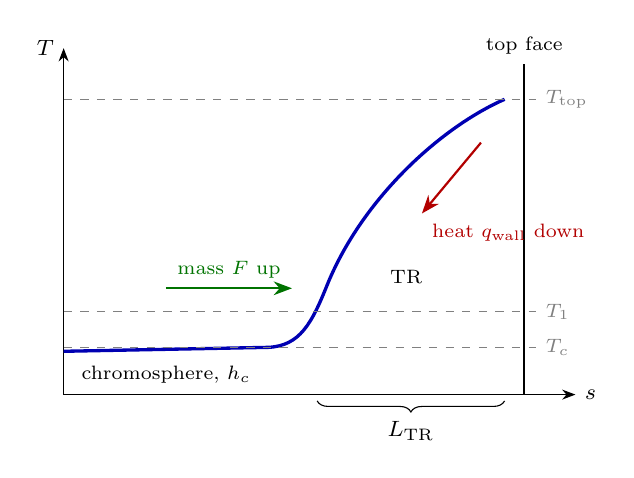
\begin{tikzpicture}[x=1cm,y=1cm,>=Stealth]
        \draw[->] (0,0) -- (6.5,0) node[right] {\footnotesize $s$};
        \draw[->] (0,0) -- (0,4.4) node[left] {\footnotesize $T$};
        \draw[very thick,blue!70!black]
          (0,0.55) -- (2.6,0.6)
          .. controls (3.0,0.62) and (3.15,0.9) .. (3.35,1.4)
          .. controls (3.8,2.5) and (4.8,3.4) .. (5.6,3.75);
        \draw[dashed,gray] (0,0.6) -- (6,0.6) node[right] {\scriptsize $T_c$};
        \draw[dashed,gray] (0,1.05) -- (6,1.05) node[right] {\scriptsize $T_1$};
        \draw[dashed,gray] (0,3.75) -- (6,3.75) node[right] {\scriptsize $\Ttop$};
        \draw[thick] (5.85,0) -- (5.85,4.2);
        \node[font=\scriptsize,above] at (5.85,4.2) {top face};
        \draw[decorate,decoration={brace,amplitude=4pt,mirror}]
          (3.22,-0.08) -- (5.6,-0.08) node[midway,below=4pt] {\footnotesize $\LTR$};
        \draw[->,thick,red!70!black] (5.3,3.2) -- (4.55,2.3)
          node[below right,font=\scriptsize] {heat $\qwall$ down};
        \draw[->,thick,green!45!black] (1.3,1.35) -- (2.9,1.35)
          node[above,midway,font=\scriptsize] {mass $F$ up};
        \node[font=\scriptsize] at (1.3,0.25) {chromosphere, $h_c$};
        \node[font=\scriptsize] at (4.35,1.5) {TR};
      \end{tikzpicture}
    \end{column}
    \begin{column}{0.40\textwidth}
      \small
      No radiation, no heating:
      \vspace{6pt}
      \begin{center}
        \fbox{\parbox{0.9\textwidth}{\centering
          heat conducted in\\ $=$\\ enthalpy carried out}}
      \end{center}
      \vspace{6pt}
      Goal: turn this into one temperature integral.
    \end{column}
  \end{columns}
\end{frame}

\begin{frame}{Roadmap of the derivation}
  \centering
  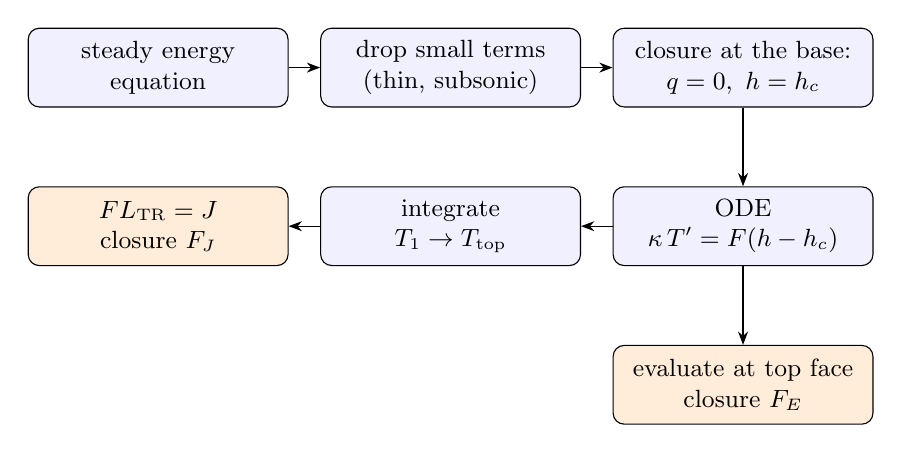
\begin{tikzpicture}[>=Stealth, node distance=4mm,
      box/.style={draw, rounded corners, fill=blue!6, align=center,
                  font=\small, minimum width=3.3cm, minimum height=1.0cm},
      clo/.style={draw, rounded corners, fill=orange!15, align=center,
                  font=\small, minimum width=3.3cm, minimum height=1.0cm}]
    \node[box] (a) {steady energy\\equation};
    \node[box, right=of a] (b) {drop small terms\\(thin, subsonic)};
    \node[box, right=of b] (c) {closure at the base:\\$q=0,\ h=h_c$};
    \node[box, below=10mm of c] (d) {ODE\\$\kappa\,T' = F(h-h_c)$};
    \node[box, left=of d] (e) {integrate\\$T_1 \to \Ttop$};
    \node[clo, left=of e] (f) {$F\LTR = J$\\closure $F_J$};
    \node[clo, below=10mm of d] (g) {evaluate at top face\\closure $F_E$};
    \draw[->] (a) -- (b); \draw[->] (b) -- (c); \draw[->] (c) -- (d);
    \draw[->] (d) -- (e); \draw[->] (e) -- (f); \draw[->] (d) -- (g);
  \end{tikzpicture}
\end{frame}

\begin{frame}{Step 1: steady state}
  Release equations, constant-area column:
  \begin{align*}
    \partial_t\rho + \partial_s F &= 0\\
    \partial_t(\rho u) + \partial_s(F u + p) &= -\rho g\\
    \partial_t\!\left(\rho e + \tfrac12\rho u^2 + \rho\phi\right)
      + \partial_s\!\left[F\left(h + \tfrac12 u^2 + \phi\right) + q\right] &= 0
  \end{align*}
  \vspace{2pt}
  Set $\partial_t = 0$ and integrate once in $s$:
  \[
    \boxed{F = \text{const}}\qquad
    \frac{dp}{ds} = -\rho g - F\frac{du}{ds}\qquad
    \boxed{F\left(h + \tfrac12u^2 + \phi\right) + q = C}
  \]
  \vspace{2pt}
  \small $h = e + p/\rho$ includes the ionization energy;\ $\phi = gs$;\
  $C$ is the total energy flux, the same at every height.
\end{frame}

\begin{frame}{Step 2: drop the small terms}
  \begin{columns}[c]
    \begin{column}{0.54\textwidth}
      \small
      Largest values in the sweep:\\[4pt]
      \begin{tabular}{@{}lll@{}}
        \toprule
        Term & Ratio & Max \\
        \midrule
        kinetic & $\tfrac12u^2/\Delta h$ & $3\times10^{-4}$ \\
        potential & $g\LTR/\Delta h$ & $0.6\,\%$ \\
        pressure & $\Delta p/p$ & few \% \\
        \bottomrule
      \end{tabular}\\[4pt]
      \scriptsize $\Delta h = \htop - h_c$; $u_{\rm top} \leq 1.39$\,km\,s$^{-1}$,
      $\mathcal{M} \leq 0.03$. Details in backup.
    \end{column}
    \begin{column}{0.44\textwidth}
      Energy:
      \[
        F\,h + q = C
      \]
      Momentum: isobaric,
      \[
        p = \ptop
      \]
      So inside the TR
      \[
        h = h(T),\qquad \kappa = \kappa(T).
      \]
    \end{column}
  \end{columns}
\end{frame}

\begin{frame}{Step 3: closure at the base of the TR}
  \textbf{Boundary condition} at the chromosphere top (cool, flat $T$):
  \[
    q \to 0,\qquad h \to h_c
    \qquad\Longrightarrow\qquad C = F\,h_c
  \]
  \vspace{4pt}
  Substitute $q = -\kappa\,dT/ds$:
  \[
    \boxed{\ \kappa(T)\,\frac{dT}{ds} = F\,\bigl[h(T) - h_c\bigr]\ }
  \]
  \vspace{4pt}
  \begin{center}
    \small heat conducted down through a level $=$ enthalpy the upflow gains
    below it
  \end{center}
\end{frame}

\begin{frame}{Step 4: solve the ODE}
  Separable, since both sides depend on $s$ only through $T$:
  \[
    ds = \frac{1}{F}\,\frac{\kappa(T)}{h(T)-h_c}\,dT
  \]
  Integrate from the marker $T_1$ to the top cell:
  \[
    \int_{s(T_1)}^{s_{\rm top}} ds
      = \frac{1}{F}\int_{T_1}^{\Ttop}\frac{\kappa}{h-h_c}\,dT
    \quad\Longrightarrow\quad
    \boxed{\ F\,\LTR = J \equiv \int_{T_1}^{\Ttop}\frac{\kappa(T,\ptop)}{h(T,\ptop)-h_c}\,dT\ }
  \]
  \vspace{2pt}
  \begin{itemize}\itemsep4pt
    \item $J$ depends only on $(\Ttop,\ \ptop,\ h_c)$.
    \item The same integral to any $T$ gives the profile:
          $s - s(T_1) = J(T)/F$.
    \item Only the product $F\LTR$ is fixed. Nothing in the release TR sets
          $\LTR$.
  \end{itemize}
\end{frame}

\begin{frame}{The closures}
  \renewcommand{\arraystretch}{1.6}
  \begin{center}
    \begin{tabular}{@{}lll@{}}
      \toprule
      & Closure & Taken from the run \\
      \midrule
      Chromosphere & $h_c = h_{\rm Saha}(T_c,\ \ptop)$,\quad $T_c = 6.7$\,kK
        & nothing \\
      Energy (ODE at top face) & $F_E = \dfrac{\qwall}{\htop - h_c}$ & $\qwall$ \\
      TR (integrated ODE) & $F_J = \dfrac{J(\Ttop,\ptop,h_c)}{\LTR}$ & $\LTR$ \\
      \bottomrule
    \end{tabular}
  \end{center}
  \vspace{6pt}
  \textbf{Tests}, each with nominal or measured $h_c$:
  \[
    \frac{\Fsim}{F_E}\ \ (=\ER\ \text{with measured } h_c)
    \qquad\qquad
    \frac{\Fsim}{F_J} = \frac{\Fsim\LTR}{J}
  \]
  \small A ratio of 1 means the simulated TR is in steady balance.
\end{frame}

\begin{frame}{Two properties of the solution}
  \begin{columns}[T]
    \begin{column}{0.48\textwidth}
      \textbf{The foot needs a marker}\\[4pt]
      Near $T_c$: $h - h_c \approx c_p(T - T_c)$, so
      \[
        T - T_c \propto e^{s/\ell},\qquad \ell = \frac{\kappa_c}{F\,c_p}
      \]
      \[
        J \sim -\frac{\kappa_c}{c_p}\ln(T_1 - T_c) \to \infty
      \]
      \small No sharp base $\Rightarrow$ fix $T_1 = 7.5$\,kK;\\
      $J$ and $\LTR$ use the same $T_1$.
    \end{column}
    \begin{column}{0.48\textwidth}
      \textbf{The hot limit}\\[4pt]
      Fully ionized: $h - h_c \approx 5\kB T/\mH$,\ $\kappa = \kappa_0T^{5/2}$:
      \[
        J \to \frac{2\,\kappa_0\,\mH}{25\,\kB}\,\Ttop^{5/2}
      \]
      \small Independent of $p$. The $p$-dependence comes from the cool part:\\
      at 70\,kK, $J/J_{\rm Spitzer} = 1.02,\ 0.88,\ 0.72$\\
      at 0.003, 0.0103, 0.08\,Pa.
    \end{column}
  \end{columns}
\end{frame}

\begin{frame}{The enthalpy: what the TR must supply}
  \[
    h = \underbrace{\tfrac52(1+x)\frac{\kB T}{\mH}}_{\text{thermal}+p/\rho}
      + \underbrace{x\,\frac{\chiH}{\mH}}_{\text{ionization}},
    \qquad \frac{\chiH}{\mH} = 1.30\times10^{9}\ \mathrm{J\,kg^{-1}}
  \]
  \vspace{2pt}
  \begin{columns}[T]
    \begin{column}{0.4\textwidth}
      \small
      \textbf{$h_c$ at 6.7\,kK} [$10^9$\,J\,kg$^{-1}$]\\[3pt]
      \begin{tabular}{@{}lrrr@{}}
        \toprule
        $\ptop$ [Pa] & $x_c$ & $h_c$ & ion. \\
        \midrule
        0.003 & 0.84 & 1.35 & 81\,\% \\
        0.0103 & 0.64 & 1.06 & 79\,\% \\
        0.08 & 0.29 & 0.55 & 68\,\% \\
        \bottomrule
      \end{tabular}
    \end{column}
    \begin{column}{0.56\textwidth}
      \small
      \textbf{$\Delta h = \htop - h_c$} [$10^9$\,J\,kg$^{-1}$] (ionization share)\\[3pt]
      \begin{tabular}{@{}lrrr@{}}
        \toprule
        $\Ttop$ & 0.003\,Pa & 0.0103\,Pa & 0.08\,Pa \\
        \midrule
        18\,kK & 0.70 (30\,\%) & 0.99 (48\,\%) & 1.50 (62\,\%) \\
        35\,kK & 1.40 (15\,\%) & 1.69 (28\,\%) & 2.20 (42\,\%) \\
        70\,kK & 2.84 (7\,\%) & 3.13 (15\,\%) & 3.64 (26\,\%) \\
        \bottomrule
      \end{tabular}
    \end{column}
  \end{columns}
  \vspace{8pt}
  \small Cool wall, high $p$: $\Delta h$ is mostly ionizing the inflow.
  Hot wall: mostly heating. Compare $\tfrac12u^2 \leq 10^{6}$\,J\,kg$^{-1}$.
\end{frame}

% ============================================================ evaluation
\section{Evaluation}

\begin{frame}{Ingredients: the release closure}
  \begin{columns}[T]
    \begin{column}{0.48\textwidth}
      \textbf{Saha, pure hydrogen}
      \[
        \frac{x^2}{1-x} = \frac{\mH}{\rho}
        \left(\frac{2\pi m_e\kB T}{h_P^2}\right)^{3/2} e^{-\chiH/\kB T}
      \]
      \[
        p = (1+x)\frac{\rho\,\kB T}{\mH}
      \]
      \small $\rho(p,T)$: fixed point
      $\rho \leftarrow p\,\mH/[(1+x)\kB T]$
    \end{column}
    \begin{column}{0.5\textwidth}
      \textbf{Conductivity} ($\kappa = \kappa_e + \kappa_n$)
      \[
        \kappa_e = \frac{9.20\times10^{-12}\,n_e\,T^{5/2}}
                        {n_e + 2.84\times10^{-11}\,n_{\rm HI}\,T^2}
      \]
      \[
        \kappa_n = \frac{0.0342\,n_{\rm HI}\,T}
          {1.21\,n_e\sqrt{2T} + 1.71\,n_{\rm HI}\sqrt{T}}
      \]
      \small Spitzer with e--H collisions, plus neutrals.
    \end{column}
  \end{columns}
  \vspace{8pt}
  \src{Same constants and formulas as \texttt{eos.hpp} and \texttt{physics.hpp};
       no TRAC, no numerical diffusivity.}
\end{frame}

\begin{frame}{Recipe}
  \begin{columns}[T]
    \begin{column}{0.55\textwidth}
      For each $(\Ttop,\ \ptop,\ T_c)$:
      \begin{enumerate}\itemsep6pt
        \item $h_c = h_{\rm Saha}(T_c,\ \ptop)$
        \item 300 log-spaced nodes, $T_1 \to \Ttop$
        \item at each node: $\rho \to x \to h,\ \kappa$
        \item trapezoidal rule for $\int \kappa/(h-h_c)\,dT$
      \end{enumerate}
    \end{column}
    \begin{column}{0.42\textwidth}
      \textbf{Table}\\[3pt]
      \small
      $\Ttop$: 29 values, 15--200\,kK\\
      $\ptop$: 33 values, $10^{-3}$--10\,Pa\\
      $T_c$: 6.0, 6.35, 6.7, 7.0\,kK\\[6pt]
      Cost: $\sim$6\,s for the whole table.
    \end{column}
  \end{columns}
\end{frame}

\begin{frame}{Anatomy of the integral ($\Ttop = 70$\,kK)}
  \centering
  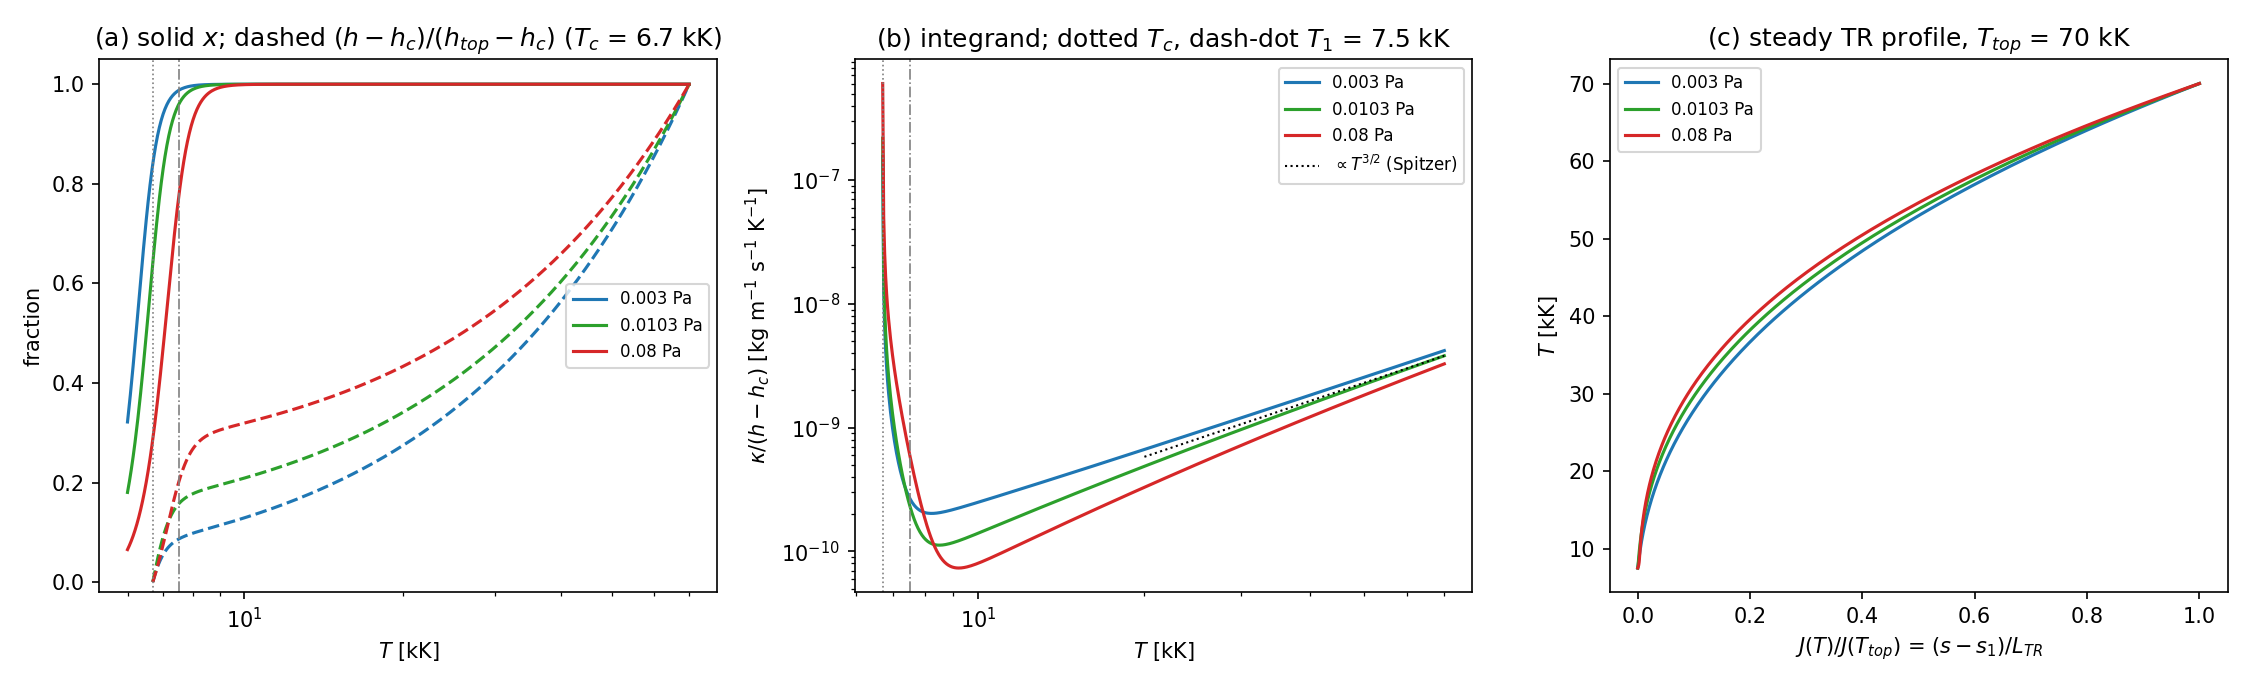
\includegraphics[width=\textwidth]{analytic_J_integrand.png}
  \vspace{2pt}
  \footnotesize
  \begin{columns}[T]
    \begin{column}{0.32\textwidth}
      (a) Higher $p$: more of $\Delta h$ gained below 10\,kK (13, 21, 32\,\%).
    \end{column}
    \begin{column}{0.32\textwidth}
      (b) Diverges at $T_c$; Spitzer $T^{3/2}$ above $\sim$20\,kK.
    \end{column}
    \begin{column}{0.32\textwidth}
      (c) Running integral $=$ steady TR profile.
    \end{column}
  \end{columns}
\end{frame}

\begin{frame}{The table}
  \begin{columns}[T]
    \begin{column}{0.5\textwidth}
      \centering
      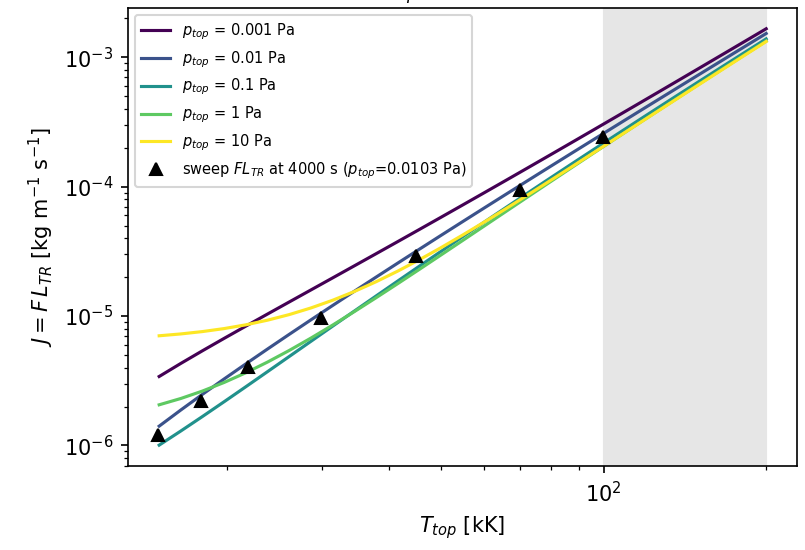
\includegraphics[width=0.8\textwidth]{Jtable_T.png}\\
      \footnotesize $J(\Ttop)$: steep, $\propto T^{2.3\text{--}3.1}$.
    \end{column}
    \begin{column}{0.5\textwidth}
      \centering
      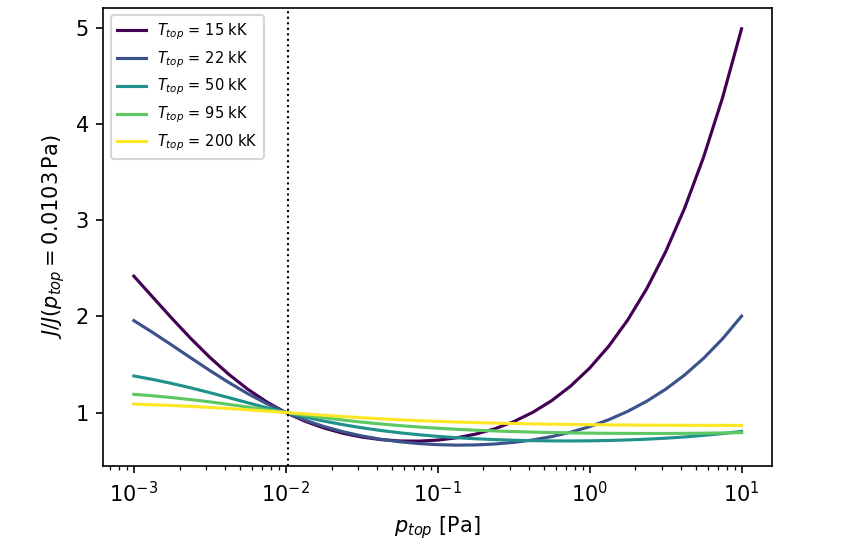
\includegraphics[width=0.8\textwidth]{Jtable_p.png}\\
      \footnotesize $J(\ptop)/J(0.0103\,\text{Pa})$: weak,
      $\partial\ln J/\partial\ln p \in [-0.39, 0.11]$.
    \end{column}
  \end{columns}
  \vspace{6pt}
  \small Exception: 15\,kK at $p > 1$\,Pa, where the ionization zone moves into
  the TR and $J$ depends on $T_1$.
\end{frame}

\begin{frame}{The hidden variable $T_c$}
  \begin{columns}[c]
    \begin{column}{0.52\textwidth}
      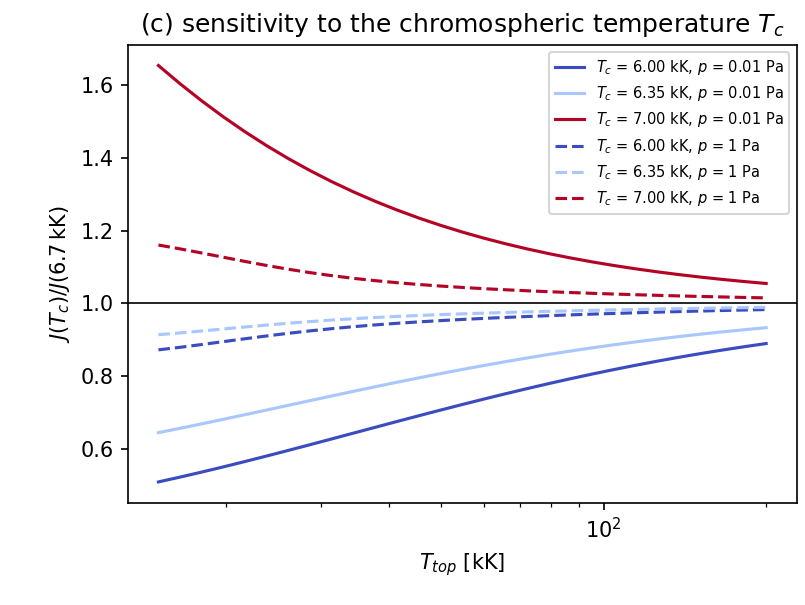
\includegraphics[width=\textwidth]{Jtable_Tc.png}
    \end{column}
    \begin{column}{0.44\textwidth}
      \small
      $J(T_c)/J(6.7\,\text{kK})$ at 22\,kK:\\[4pt]
      \begin{tabular}{@{}lrr@{}}
        \toprule
        $T_c$ & 0.0103\,Pa & 1\,Pa \\
        \midrule
        6.35\,kK & 0.70 & 0.94 \\
        7.0\,kK & 1.47 & 1.06 \\
        \bottomrule
      \end{tabular}\\[8pt]
      Sensitive at low $p$, where $x_c$ is mid-ionization.\\[4pt]
      AWSoM does not supply $T_c$.
    \end{column}
  \end{columns}
\end{frame}

% ============================================================ sweep setting
\section{The sweep}

\begin{frame}{Setup}
  \begin{columns}[T]
    \begin{column}{0.48\textwidth}
      \textbf{Canonical release}\\[4pt]
      \small
      N=500/R4, 661 cells, 1600--2153\,km\\
      fine cells 0.276\,km; grade 2079--2101\,km\\
      Godunov + implicit physical conduction\\
      CFL 0.50, double precision\\[8pt]
      \textbf{Runs}\\[4pt]
      5000\,s, snapshots every 10\,s\\
      all 31: \texttt{end\_time}, 0 fallbacks
    \end{column}
    \begin{column}{0.48\textwidth}
      \textbf{Two knobs}\\[4pt]
      \begin{tabular}{@{}ll@{}}
        \toprule
        \texttt{ISO\_T\_TOP} & 18, 25, 35, 50, 70\,kK \\
        \texttt{ISO\_P\_TOP} & 0.003, 0.005, 0.0103,\\
          & 0.02, 0.04, 0.08\,Pa \\
        \bottomrule
      \end{tabular}\\[8pt]
      \small
      30 runs + one N=1000 control\\ (50\,kK, 0.0103\,Pa).\\[10pt]
      \begin{block}{Release point}
        \footnotesize
        $\Twall = 22$\,kK\quad(\texttt{ISO\_T\_TOP=22000})\\
        $\ptop = 0.0103$\,Pa\quad(C7 top cell; \texttt{kOuterPRef})\\[3pt]
        0.0103\,Pa is a sweep column; 22\,kK is \emph{not} a sweep row. It
        sits between the 18 and 25\,kK runs.
      \end{block}
    \end{column}
  \end{columns}
\end{frame}

\begin{frame}{How $\Twall$ and $\ptop$ are changed}
  \begin{columns}[T]
    \begin{column}{0.42\textwidth}
      \textbf{$\Twall$: \texttt{ISO\_T\_TOP} [K]}\\[4pt]
      \small
      Boundary only.
      \begin{itemize}\itemsep4pt
        \item Sets the fixed temperature of both outer hydro ghosts.
        \item Conduction reads the same value as its Dirichlet datum.
        \item IC unchanged: the C7 column.
      \end{itemize}
      \vspace{4pt}
      The IC top cell ($\approx 22.6$\,kK) and the wall disagree at $t=0$;
      that mismatch drives the run.
    \end{column}
    \begin{column}{0.54\textwidth}
      \textbf{$\ptop$: \texttt{ISO\_P\_TOP} [Pa]}\\[4pt]
      \small
      Whole column rebuilt.
      \begin{enumerate}\itemsep3pt
        \item Keep the C7 $T(h)$.
        \item Integrate $\dfrac{d\ln p}{dh} = -\dfrac{g\,\mH}{(1+x)\,\kB T}$
              up from a trial $p_b$.
        \item Secant on $\ln p_b$ until the top cell is at $\ptop$.
        \item Both reservoirs (\texttt{kOuterPRef}, inner) from the rebuilt
              column.
      \end{enumerate}
      \vspace{3pt}
      \footnotesize
      $\ptop = 0.003$\,Pa: $p_b = 0.0151$\,Pa ($0.22\times$ C7)\\
      $\ptop = 0.08$\,Pa: $p_b = 0.822$\,Pa ($12.1\times$ C7)\\[3pt]
      Initial $\LTR$ and $T_c$ stay at the C7 values.
    \end{column}
  \end{columns}
  \vspace{8pt}
  \scriptsize One case (\texttt{util/run\_tp\_sweep.sh} runs 4 at a time):\\[2pt]
  \texttt{ISO\_T\_TOP=50000 ISO\_P\_TOP=0.02 CHROMO\_T\_END=5000 scripts/run\_chromo\_realtime.sh
    out.txt full no-ionization model\_column - 20.0 no-cooling}
\end{frame}

\begin{frame}{What is measured, and when}
  \begin{columns}[T]
    \begin{column}{0.52\textwidth}
      \small
      \begin{tabular}{@{}ll@{}}
        \toprule
        $\Fsim$ & top-cell $\rho u$ \\
        $\qwall$ & top-face conductive flux \\
        $\LTR$ & top cell $-$ 7.5\,kK isotherm \\
        measured $h_c$ & first cell below 7.5\,kK \\
         & with $|q| < 1\,\%\ \qwall$ \\
        \bottomrule
      \end{tabular}
    \end{column}
    \begin{column}{0.46\textwidth}
      \small
      $t_{\rm ready}$ = later of:
      \begin{itemize}
        \item $|F_{\rm base}/F_{\rm top}-1| < 5\,\%$
        \item $\ER$ within 0.05 of its end value
      \end{itemize}
      \vspace{4pt}
      Read: 300\,s from $t_{\rm ready}$, and 4700--5000\,s (``end'').\\
      $\ast$ = not ready before 5000\,s.
    \end{column}
  \end{columns}
  \vspace{10pt}
  \small\textbf{Classes} (from flux statistics after 1000\,s):\\[3pt]
  \colorbox{unsteady}{unsteady}: $\max_z \mathrm{std}_t F/|\mathrm{mean}_t F| > 0.5$
  \quad
  \colorbox{relaxing}{relaxing}: $\ER > 1.03$, still falling
  \quad
  \colorbox{relaxed}{relaxed}: the rest
\end{frame}

% ============================================================ results
\section{Results}

\begin{frame}{The map}
  \begin{columns}[c]
    \begin{column}{0.56\textwidth}
      \centering
      \renewcommand{\arraystretch}{1.5}
      \footnotesize
      \setlength{\tabcolsep}{4pt}
      \begin{tabular}{r|cccccc}
        $\Twall$ & \multicolumn{6}{c}{$\ptop$ [Pa]} \\
        {[kK]} & 0.003 & 0.005 & 0.0103 & 0.02 & 0.04 & 0.08 \\
        \hline
        70 & \cellcolor{relaxed}.981 & \cellcolor{relaxed}.979 & \cellcolor{relaxed}.977
           & \cellcolor{unsteady}.943$^\ast$ & \cellcolor{unsteady}1.061$^\ast$ & \cellcolor{unsteady}1.042$^\ast$ \\
        50 & \cellcolor{relaxed}.971 & \cellcolor{relaxed}.970 & \cellcolor{relaxed}.968
           & \cellcolor{relaxed}.964$^\ast$ & \cellcolor{unsteady}.966$^\ast$ & \cellcolor{unsteady}.952$^\ast$ \\
        35 & \cellcolor{relaxed}.955 & \cellcolor{relaxed}.952 & \cellcolor{relaxed}.950
           & \cellcolor{relaxed}.953 & \cellcolor{relaxed}.961 & \cellcolor{relaxed}.992 \\
        25 & \cellcolor{relaxed}.933 & \cellcolor{relaxed}.935 & \cellcolor{relaxed}.966
           & \cellcolor{relaxed}.984 & \cellcolor{relaxing}1.031 & \cellcolor{relaxing}1.128 \\
        \textcolor{release}{\textbf{22}} & & & \textcolor{release}{$\bigstar$\,\textbf{release}} & & & \\
        18 & \cellcolor{relaxed}.928 & \cellcolor{relaxed}.934 & \cellcolor{relaxed}.955
           & \cellcolor{relaxed}.988 & \cellcolor{relaxing}1.042 & \cellcolor{relaxing}1.174 \\
      \end{tabular}\\[6pt]
      \scriptsize $\ER$ at $t_{\rm ready}$.\quad
      \colorbox{relaxed}{relaxed 21}\ \colorbox{relaxing}{relaxing 4}\
      \colorbox{unsteady}{unsteady 5}\\[3pt]
      \textcolor{release}{$\bigstar$} release (22\,kK, 0.0103\,Pa): not rerun here;
      bracketed by .955 and .966.
    \end{column}
    \begin{column}{0.40\textwidth}
      \small
      \begin{itemize}\itemsep8pt
        \item Most of the plane: $\ER = 0.93$--$0.99$.
        \item Cool wall, high $p$: upper bounds.
        \item Hot wall, high $p$: noisy, mean right.
        \item \textcolor{release}{Release point}: inside the quiet, relaxed
              region.
      \end{itemize}
    \end{column}
  \end{columns}
\end{frame}

\begin{frame}{$J$: simulation against the integral}
  \begin{columns}[T]
    \begin{column}{0.5\textwidth}
      \centering
      \relfig{0.8\textwidth}{sweep_J_vs_p.png}{0.490}{0.118}{0.995}\\
      \footnotesize Markers: $F\LTR$. Lines: integral, nominal $T_c$.
    \end{column}
    \begin{column}{0.5\textwidth}
      \centering
      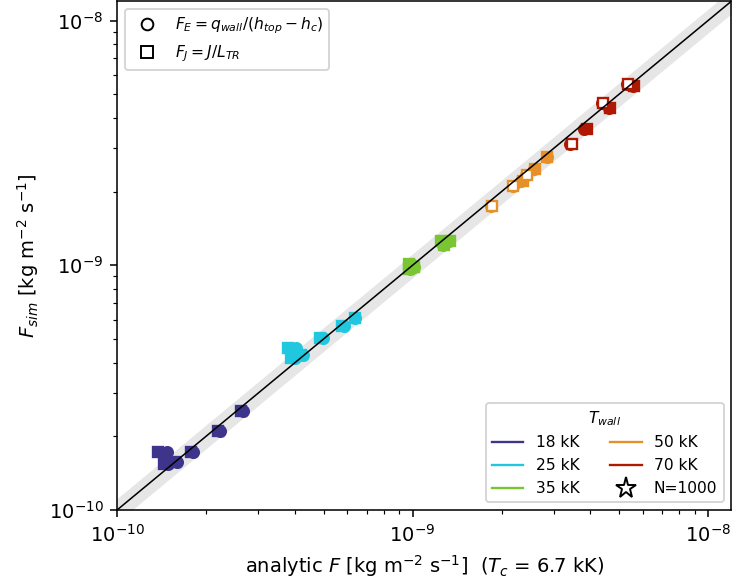
\includegraphics[width=0.8\textwidth]{sweep_parity.png}\\
      \footnotesize $\Fsim$ vs $F_E$ ($\circ$) and $F_J$ ($\square$); band
      $\pm10\,\%$.
    \end{column}
  \end{columns}
  \vspace{4pt}
  \footnotesize Colours: \textcolor[RGB]{60,50,140}{18},
  \textcolor[RGB]{30,190,220}{25}, \textcolor[RGB]{110,190,40}{35},
  \textcolor[RGB]{230,140,40}{50}, \textcolor[RGB]{180,20,10}{70}\,kK.
  Open: not ready. Star: N=1000.
  \textcolor{release}{Release: 22\,kK, between the 18 and 25\,kK curves.}
\end{frame}

\begin{frame}{Result 1: the energy closure holds at every pressure}
  \begin{columns}[c]
    \begin{column}{0.54\textwidth}
      \relfig{\textwidth}{sweep_ER.png}{0.4785}{0.1436}{0.99}\\
      \centering\footnotesize $\ER$ (measured $h_c$).
      $\bullet$ $t_{\rm ready}$, $\times$ end. Grey: $\pm5\,\%$.
    \end{column}
    \begin{column}{0.42\textwidth}
      \small
      Relaxed runs:\\[4pt]
      \begin{tabular}{@{}lrr@{}}
        \toprule
        & $t_{\rm ready}$ & end \\
        \midrule
        $\ER$ & 0.93--0.99 & 0.90--0.98 \\
        $F L/J$, nom. & 0.93--1.03 & 0.84--1.01 \\
        \bottomrule
      \end{tabular}\\[8pt]
      $\ER < 1$ always: 1--10\,\% of the heat goes elsewhere, mainly into
      ionizing the gas the growing TR absorbs.\\[6pt]
      \textcolor{release}{Release bracket} (18 / 25\,kK at 0.0103\,Pa):
      $\ER = 0.955 / 0.966$, end $0.913 / 0.930$.
    \end{column}
  \end{columns}
\end{frame}

\begin{frame}{Result 2: a fixed-$T_c$ table drifts low at low $p$}
  \begin{columns}[T]
    \begin{column}{0.5\textwidth}
      \centering
      \relfig{0.7\textwidth}{sweep_FLJ_nom.png}{0.4651}{0.1436}{0.99}\\
      \footnotesize $F\LTR/J$, nominal $T_c$ ($\times$: end).
    \end{column}
    \begin{column}{0.5\textwidth}
      \centering
      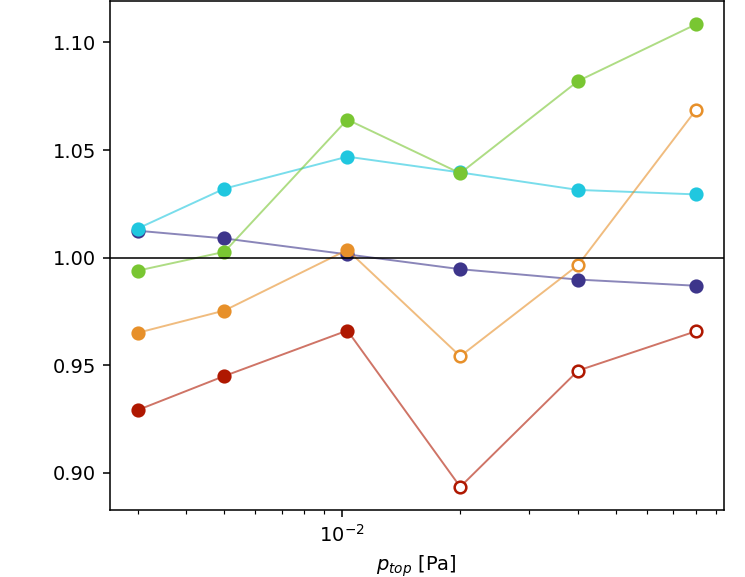
\includegraphics[width=0.7\textwidth]{sweep_hc_ratio.png}\\
      \footnotesize measured $h_c$ / nominal $h_c$, $t_{\rm ready}$.
    \end{column}
  \end{columns}
  \vspace{4pt}
  \small
  \begin{tabular}{@{}lll@{}}
    At 5000\,s: & $F L/J$ nominal & $0.84$--$0.92$ at $\ptop \leq 0.0103$\,Pa \\
    & $h_c/h_c^{\rm nom}$ & down to $0.80$ (70\,kK, 0.003\,Pa) \\
    & $\ER$, measured $h_c$ & still $0.98$ there \\
    \textcolor{release}{Release bracket:} & $F L/J$ nominal, end & $0.905$ (18\,kK),
      $0.917$ (25\,kK): inside the drift \\
  \end{tabular}
\end{frame}

\begin{frame}{Why the $T_c$ drift happens}
  \centering
  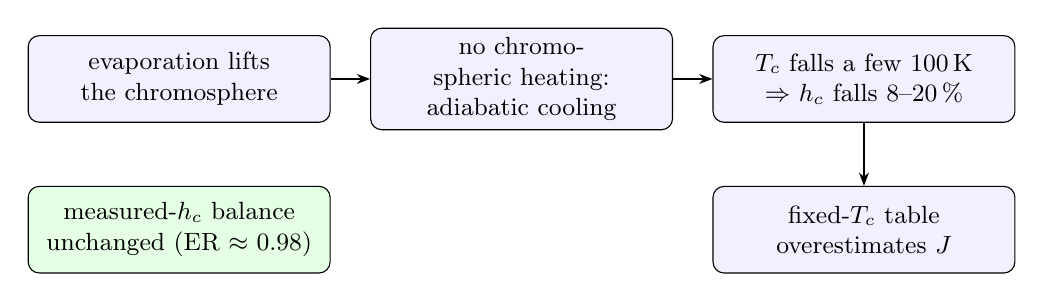
\begin{tikzpicture}[>=Stealth, node distance=5mm,
      box/.style={draw, rounded corners, fill=blue!6, align=center,
                  font=\small, text width=3.6cm, minimum height=1.1cm}]
    \node[box] (a) {evaporation lifts\\the chromosphere};
    \node[box, right=of a] (b) {no chromospheric heating:\\adiabatic cooling};
    \node[box, right=of b] (c) {$T_c$ falls a few 100\,K\\$\Rightarrow$ $h_c$ falls 8--20\,\%};
    \node[box, below=8mm of c] (d) {fixed-$T_c$ table\\overestimates $J$};
    \node[box, below=8mm of a, fill=green!10] (e) {measured-$h_c$ balance\\unchanged ($\ER \approx 0.98$)};
    \draw[->] (a) -- (b); \draw[->] (b) -- (c); \draw[->] (c) -- (d);
  \end{tikzpicture}
  \vspace{10pt}

  \small Largest in hot, low-$p$ runs: fastest evaporation relative to column
  mass ($\LTR$: 30 $\to$ 62\,km at 70\,kK, 0.003\,Pa).\\[4pt]
  The TR physics is fine; only the table's assumed $T_c$ is wrong.
\end{frame}

\begin{frame}{Result 3: cool wall, high $p$ --- the TR outlasts the run}
  \centering
  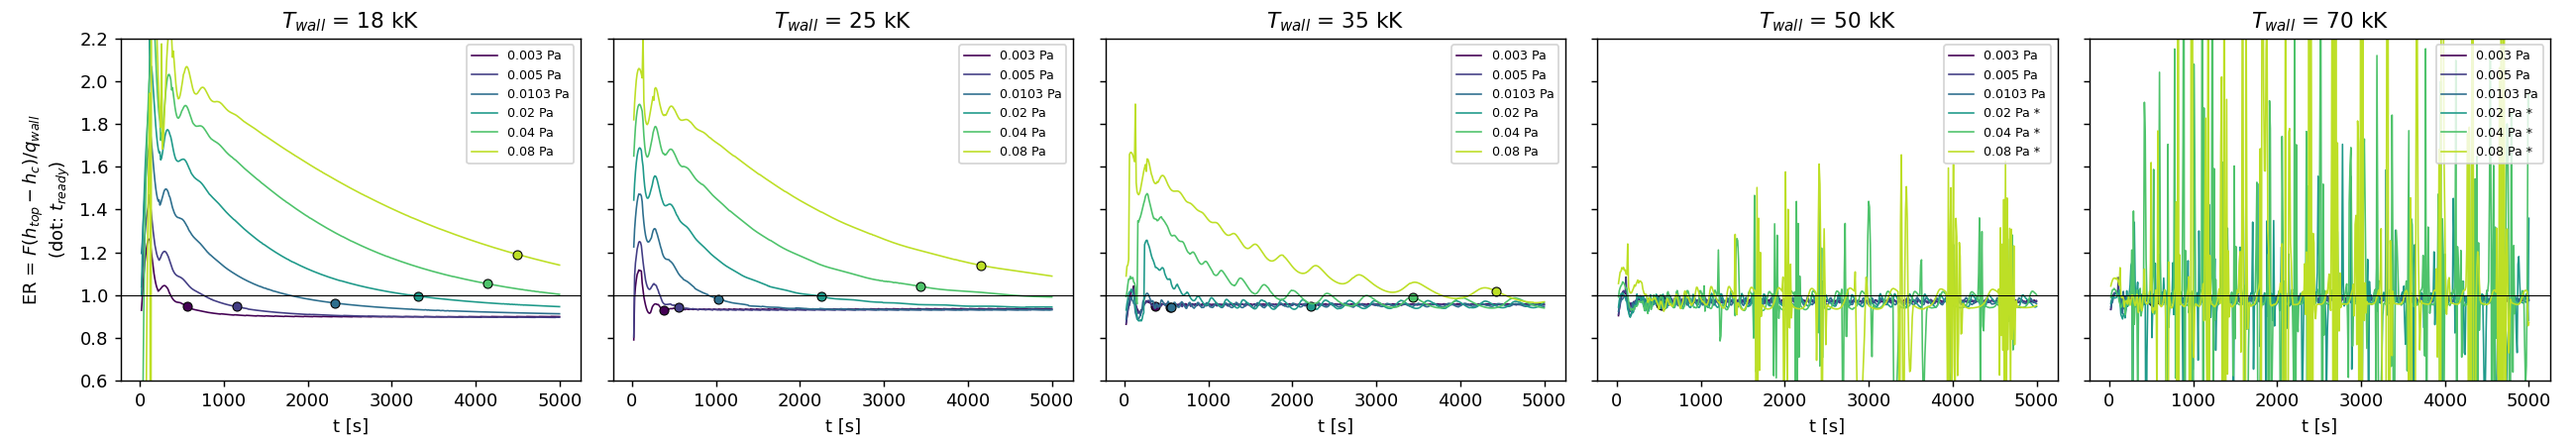
\includegraphics[width=\textwidth]{series_ER.png}\\
  \vspace{2pt}
  \begin{columns}[T]
    \begin{column}{0.44\textwidth}
      \small
      Initial C7 TR: $\ER \approx 1.5$--2.\\
      Drains slower at higher $p$.\\[4pt]
      4 runs still falling at 5000\,s\\ $\Rightarrow$ upper bounds.
    \end{column}
    \begin{column}{0.52\textwidth}
      \scriptsize
      \begin{tabular}{@{}lrrrrrr@{}}
        \toprule
        $\tau$ [s] & .003 & .005 & .0103 & .02 & .04 & .08\,Pa \\
        \midrule
        18\,kK & 370 & 650 & 880 & 1100 & 1850 & 3450 \\
        25\,kK & -- & -- & 440 & 820 & 1190 & 2100 \\
        35\,kK & -- & -- & -- & -- & 630 & 1270 \\
        \bottomrule
      \end{tabular}\\[2pt]
      Fit $\ER = a + b\,e^{-t/\tau}$ from 1000\,s.
    \end{column}
  \end{columns}
\end{frame}

\begin{frame}{Result 4: hot wall, high $p$ --- N500 is unsteady}
  \centering
  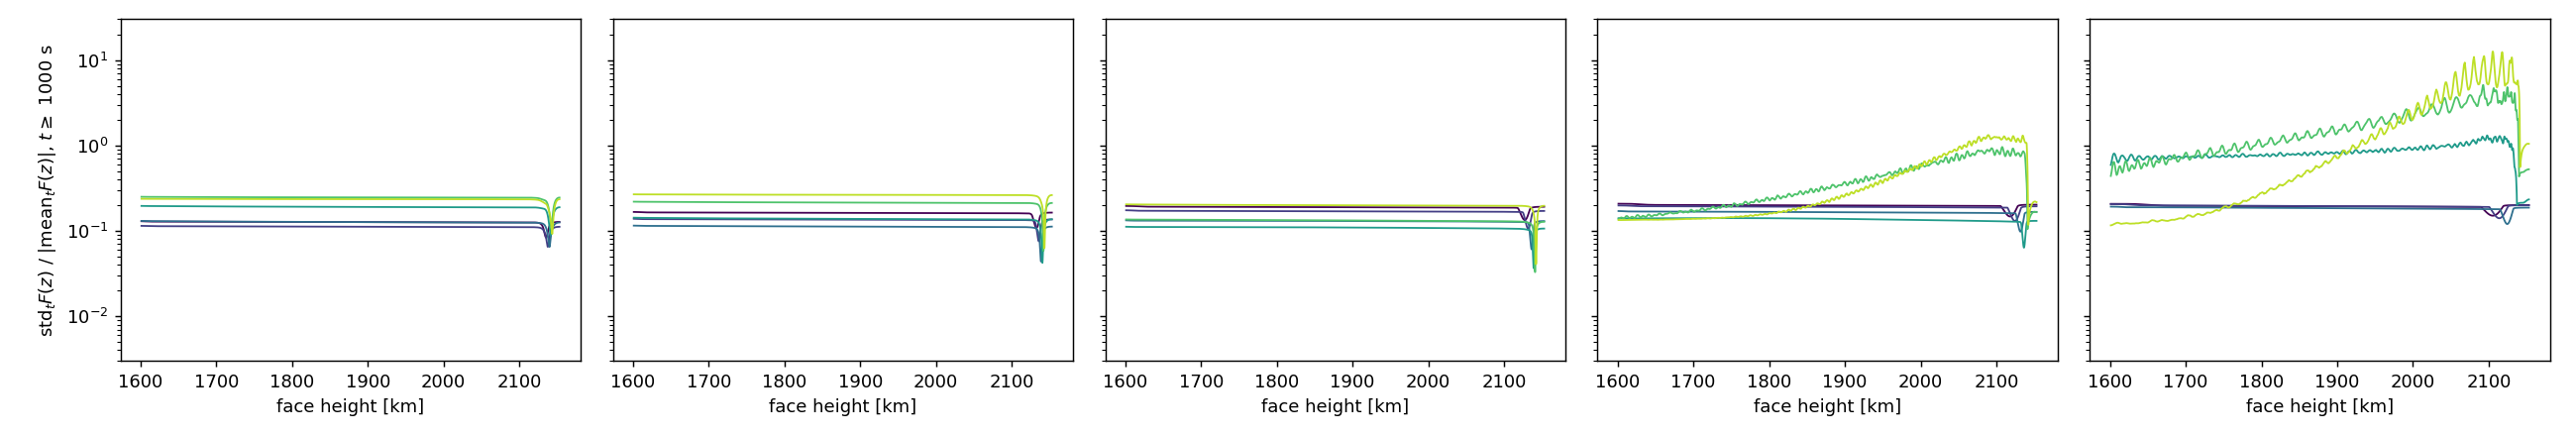
\includegraphics[width=\textwidth]{series_unsteady.png}\\
  \footnotesize $\mathrm{std}_t F(z)/|\mathrm{mean}_t F(z)|$ vs height, after
  1000\,s. Panels: 18 $\to$ 70\,kK.
  \vspace{6pt}
  \begin{columns}[T]
    \begin{column}{0.48\textwidth}
      \small
      50\,kK at 0.04, 0.08\,Pa\\
      70\,kK at 0.02, 0.04, 0.08\,Pa
    \end{column}
    \begin{column}{0.48\textwidth}
      \small
      70\,kK, 0.08\,Pa: top face reverses in 75/893 captures.\\
      300\,s means of $\ER$: 0.91--1.06.
    \end{column}
  \end{columns}
\end{frame}

\begin{frame}{Corner follow-up: 70\,kK, 0.08\,Pa, 1500\,s}
  \footnotesize
  \begin{center}
    \begin{tabular}{@{}lrrrrr@{}}
      \toprule
      Variant & cell [km] & peak unsteadiness & top $F\leq0$ &
        mean $F$ [$10^{-9}$] & $\ER$ \\
      \midrule
      N500, CFL 0.50 & 0.276 & 6.7 & 9.0\,\% & 6.89 & $0.985\pm0.79$ \\
      CFL 0.25 & 0.276 & 7.2 & 9.2\,\% & 6.91 & $0.984\pm1.02$ \\
      grade moved to 1950\,km & 0.276 & 7.2 & 5.0\,\% & 6.97 & $1.007\pm1.01$ \\
      \rowcolor{relaxed} N1000 & 0.138 & 1.7 & 0 & 6.88 & $0.975\pm0.25$ \\
      \bottomrule
    \end{tabular}
  \end{center}
  \vspace{6pt}
  \small
  \begin{tabular}{@{}ll@{}}
    time step & not the cause (same bursts) \\
    mesh grade & not the cause (same bursts) \\
    resolution & controls it ($4\times$ weaker, no reversals) \\
    mean flux & same to 1.5\,\% in all four \\
  \end{tabular}
\end{frame}

\begin{frame}{Follow-up in pictures}
  \begin{columns}[T]
    \begin{column}{0.5\textwidth}
      \centering
      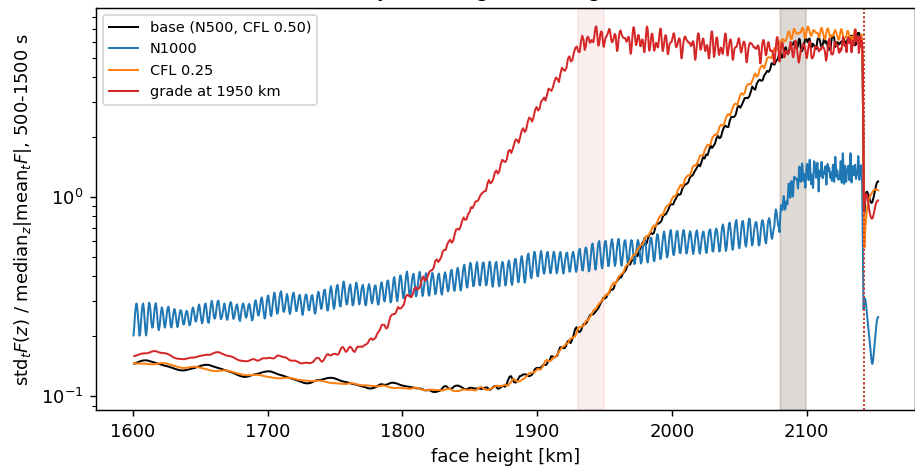
\includegraphics[width=\textwidth]{corner_std_profile.png}\\
      \footnotesize Where $F$ is unsteady. Shading: grade; dotted: TR base.
    \end{column}
    \begin{column}{0.5\textwidth}
      \centering
      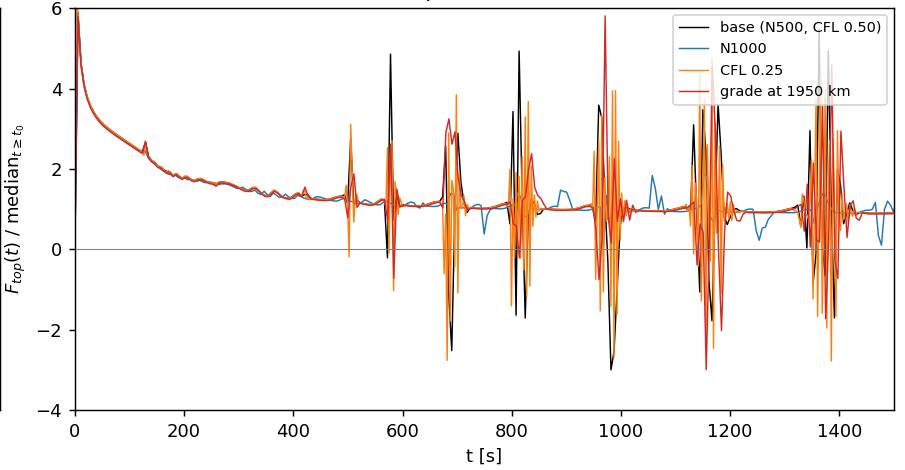
\includegraphics[width=\textwidth]{corner_top_flux.png}\\
      \footnotesize Top-face $F$. Black, orange, red burst together; blue
      (N1000) barely.
    \end{column}
  \end{columns}
\end{frame}

\begin{frame}{Follow-up: $F(z,t)$}
  \centering
  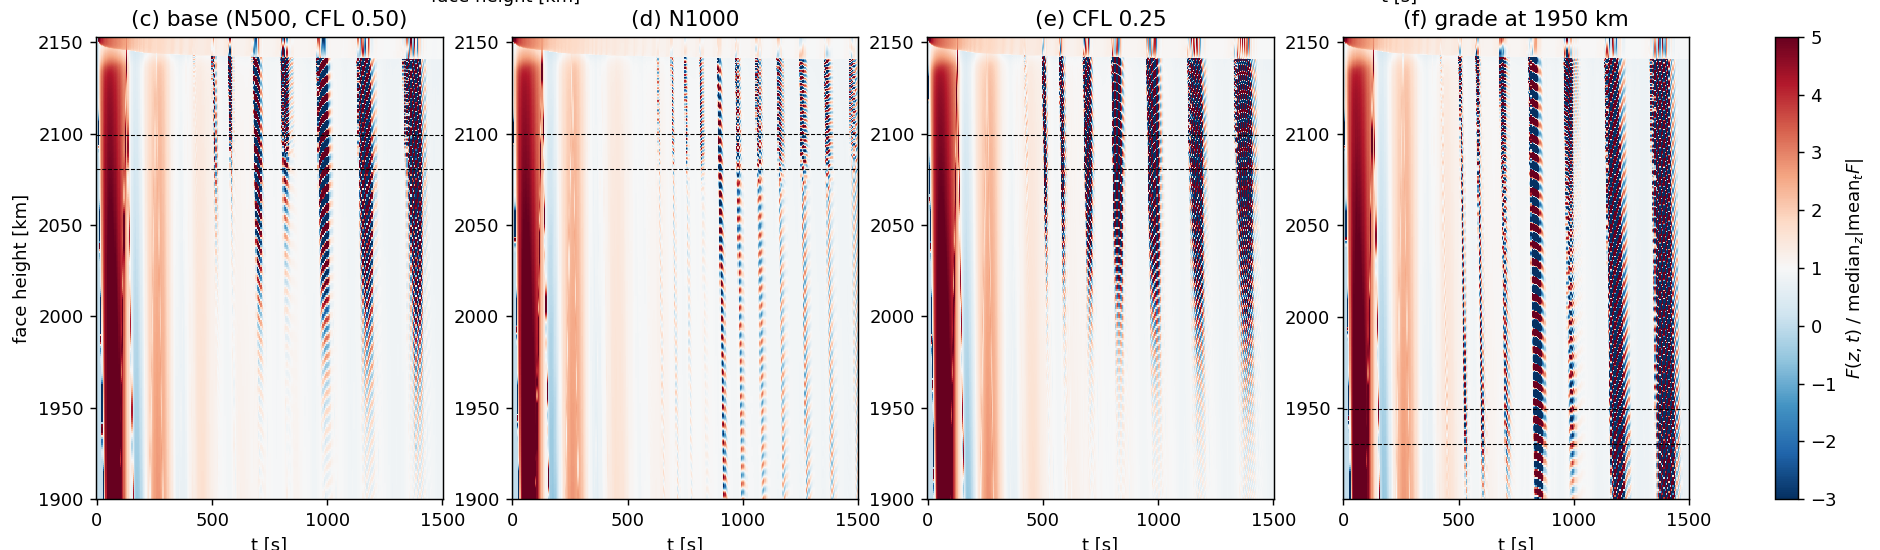
\includegraphics[width=\textwidth]{corner_spacetime.png}\\
  \vspace{4pt}
  \small Baseline, N1000, CFL 0.25, moved grade. Bursts start at the TR.
\end{frame}

\begin{frame}{The bursts are locked to the grid}
  \begin{columns}[T]
    \begin{column}{0.5\textwidth}
      \textbf{Timing}\\[4pt]
      \small
      \begin{tabular}{@{}lrrrr@{}}
        \toprule
        7\,kK enters a cell [s] & 800 & 970 & 1150 & 1370 \\
        burst starts [s] & 802 & 959 & 1133 & 1340 \\
        \bottomrule
      \end{tabular}\\[4pt]
      (7.5\,kK crossings do not match.)
    \end{column}
    \begin{column}{0.46\textwidth}
      \textbf{Width}: the foot is sub-cell\\[4pt]
      \small
      \begin{tabular}{@{}lrr@{}}
        \toprule
        & 7.0--7.5\,kK & cell \\
        \midrule
        N500 & 0.18\,km & 0.276\,km \\
        N1000 & 0.12\,km & 0.138\,km \\
        \bottomrule
      \end{tabular}\\[4pt]
      steady integral: 0.13--0.14\,km
    \end{column}
  \end{columns}
  \vspace{12pt}
  \begin{center}
    \small An under-resolved front crossing cell faces.\\ A physical
    instability would not weaken $4\times$ under refinement.
  \end{center}
\end{frame}

\begin{frame}{Open questions about the corner}
  \begin{itemize}\itemsep10pt
    \item \textbf{Why only high $p$?} Low-$p$ hot runs have even thinner feet
          ($\sim$0.05\,km) and stay quiet.
    \item \textbf{Untested candidate:} share of $\Delta h$ gained in the foot
          (6.7--10\,kK), at 70\,kK: 0.13 $\to$ 0.32 from 0.003 to 0.08\,Pa.
    \item \textbf{N1000 is not noise-free} (1.7 vs $\leq 0.27$ quiet). N2000
          not run.
    \item \textbf{TRAC} would address it, but is a design decision.
  \end{itemize}
\end{frame}

\begin{frame}{Resolution check elsewhere: 50\,kK, 0.0103\,Pa}
  \vfill
  \begin{columns}[c]
    \begin{column}{0.55\textwidth}
      \begin{tabular}{@{}lrr@{}}
        \toprule
        & N=500 & N=1000 \\
        \midrule
        $\Fsim$ [$10^{-9}$] & 2.774 & 2.780 \\
        $\LTR$ [km] & 14.4 & 14.5 \\
        $\ER$ & 0.968 & 0.966 \\
        $F L/J$, nom. & 0.970 & 0.968 \\
        \bottomrule
      \end{tabular}
    \end{column}
    \begin{column}{0.42\textwidth}
      \small
      0.2\,\% in $F$.\\[6pt]
      One point only: N500 long-run flux still not shown converged to
      $<10\,\%$.
    \end{column}
  \end{columns}
  \vfill
\end{frame}

% ============================================================ implications
\section{Implications}

\begin{frame}{For an AWSoM-R lookup}
  \begin{itemize}\itemsep10pt
    \item \textbf{Usable} over 18--70\,kK $\times$ 0.003--0.08\,Pa, 2--10\,\%
          low, \emph{if $h_c$ is right}.
    \item \textbf{Tabulate $J$}, not $F$: $\LTR$ is not set by TR physics.
    \item \textbf{$T_c$ is the weak link}: table dimension or fixed model
          choice.
    \item \textbf{Hot, high-$p$ corner:} N500 valid as a $\gtrsim 500$\,s
          mean; instantaneous needs N1000.
    \item \textbf{Cool, high-$p$ corner:} upper bounds until a $\sim$10\,ks run
          or a balanced initial TR.
  \end{itemize}
\end{frame}

\begin{frame}{Limits}
  \begin{itemize}\itemsep10pt
    \item Release physics only: no radiation, no heating, Saha $h_c$.
    \item Initial TR is C7-shaped at every $p$.
    \item Not a coupled test: AWSoM-R's TR is static and radiative
          (Sokolov et al.\ 2021).
    \item Each closure borrows one run quantity ($\qwall$ or $\LTR$).
    \item No plateau: $F$ drifts 1--6\,\% per 500\,s; quote $J$ with reading
          time.
  \end{itemize}
\end{frame}

\begin{frame}{Summary}
  \vfill
  \begin{enumerate}\itemsep12pt
    \item Steady release TR: $\kappa\,T' = F(h-h_c)$ $\Rightarrow$
          $F\LTR = J(\Ttop,\ptop,h_c)$.
    \item 31 runs, all clean. Quiet runs: $\ER = 0.93$--$0.99$ across
          $27\times$ in pressure.
    \item Fixed-$T_c$ table drifts low at low $p$ because $T_c$ falls; the
          balance does not.
    \item Two flagged corners: still relaxing (cool, high $p$); grid-scale
          bursts with correct mean (hot, high $p$).
  \end{enumerate}
  \vfill
\end{frame}

% ============================================================ backup
\appendix

\begin{frame}{Backup: size of the neglected terms}
  \footnotesize
  \begin{center}
    \begin{tabular}{@{}llll@{}}
      \toprule
      Term & Ratio & Largest & Where \\
      \midrule
      kinetic energy & $\tfrac12u_{\rm top}^2/\Delta h$ & $3.4\times10^{-4}$ &
        70\,kK, 0.003\,Pa \\
      potential energy & $g\LTR/\Delta h$ & $0.6\,\%$ & 18\,kK, 0.003\,Pa \\
      inertia & $\mathcal{M}^2$ & $1.0\times10^{-3}$ & 70\,kK, 0.003\,Pa \\
      hydrostatic drop & $\int ds/H$ & few \% & $H$: 380\,km at base, Mm when hot \\
      \bottomrule
    \end{tabular}
  \end{center}
  \vspace{6pt}
  \begin{tabular}{@{}ll@{}}
    $u_{\rm top} = \Fsim/\rho_{\rm top}$ & $\rho_{\rm top}$ from Saha at the
      top-cell $(T,p)$ \\
    reading window & 1.39\,km\,s$^{-1}$ (70\,kK, 0.003\,Pa) \\
    after 1000\,s, max & 1.24\,km\,s$^{-1}$ \\
    first 10\,s snapshot & 3.3\,km\,s$^{-1}$ (start-up transient) \\
    18\,kK, 0.08\,Pa & $\approx 1$\,m\,s$^{-1}$ \\
    $c_s = \sqrt{\tfrac53 p/\rho}$ & 22--44\,km\,s$^{-1}$ \\
  \end{tabular}
\end{frame}

\begin{frame}{Backup: full enthalpy breakdown [$10^9$\,J\,kg$^{-1}$]}
  \small
  \[
    h = \tfrac32(1+x)\frac{\kB T}{\mH} + (1+x)\frac{\kB T}{\mH} + x\frac{\chiH}{\mH},
    \qquad \frac{\kB}{\mH} = 8254\ \mathrm{J\,kg^{-1}\,K^{-1}}
  \]
  \begin{center}
    \begin{tabular}{@{}lrrrrr@{}}
      \toprule
      $T$, $p$ & $x$ & thermal & $p/\rho$ & ionization & $h$ \\
      \midrule
      6.7\,kK, 0.003\,Pa & 0.84 & 0.153 & 0.102 & 1.094 & 1.348 \\
      6.7\,kK, 0.0103\,Pa & 0.64 & 0.136 & 0.091 & 0.834 & 1.061 \\
      6.7\,kK, 0.08\,Pa & 0.29 & 0.107 & 0.071 & 0.373 & 0.551 \\
      \midrule
      10\,kK (any sweep $p$) & 1.00 & 0.248 & 0.165 & 1.303 & 1.716 \\
      18\,kK & 1 & 0.446 & 0.297 & 1.303 & 2.046 \\
      35\,kK & 1 & 0.867 & 0.578 & 1.303 & 2.748 \\
      70\,kK & 1 & 1.733 & 1.156 & 1.303 & 4.192 \\
      \bottomrule
    \end{tabular}
  \end{center}
\end{frame}

\begin{frame}{Backup: all 31 runs}
  \tiny
  \setlength{\tabcolsep}{3.2pt}
  \renewcommand{\arraystretch}{0.82}
  \begin{center}
  \begin{tabular}{@{}rrlrrrrrrrrrr@{}}
    \toprule
    $\Twall$ & $\ptop$ & class & $t_{\rm ready}$ & $\Fsim$ & $\LTR$ & $\ER$ & $\ER$ &
      $\Fsim/F_E$ & nom & $FL/J$ & nom & $h_c/h_c^{\rm nom}$ \\
    kK & Pa & & s & kg\,m$^{-2}$\,s$^{-1}$ & km & & end & nom & end & nom & end & end \\
    \midrule
18 & 0.003 & relaxed & 560 & 2.546e-10 & 14.1 & 0.928 & 0.899 & 0.951 & 0.864 & 0.967 & 0.837 & 0.979 \\
18 & 0.005 & relaxed & 1150 & 2.107e-10 & 14.0 & 0.934 & 0.895 & 0.948 & 0.878 & 0.959 & 0.862 & 0.988 \\
18 & 0.0103 & relaxed & 2330 & 1.727e-10 & 13.4 & 0.955 & 0.913 & 0.957 & 0.909 & 0.968 & 0.905 & 0.996 \\
18 & 0.02 & relaxed & 3310 & 1.574e-10 & 12.6 & 0.988 & 0.948 & 0.984 & 0.942 & 1.001 & 0.947 & 0.993 \\
18 & 0.04 & relaxing & 4140 & 1.547e-10 & 12.0 & 1.042 & 1.010 & 1.036 & 1.004 & 1.069 & 1.025 & 0.989 \\
18 & 0.08 & relaxing & 4500 & 1.731e-10 & 11.9 & 1.174 & 1.154 & 1.169 & 1.149 & 1.261 & 1.231 & 0.987 \\
25 & 0.003 & relaxed & 384 & 6.070e-10 & 13.8 & 0.933 & 0.935 & 0.951 & 0.885 & 0.953 & 0.853 & 0.958 \\
25 & 0.005 & relaxed & 554 & 5.667e-10 & 13.2 & 0.935 & 0.931 & 0.970 & 0.900 & 0.984 & 0.880 & 0.970 \\
25 & 0.0103 & relaxed & 1030 & 5.025e-10 & 12.7 & 0.966 & 0.930 & 1.006 & 0.925 & 1.032 & 0.917 & 0.993 \\
25 & 0.02 & relaxed & 2260 & 4.303e-10 & 12.6 & 0.984 & 0.944 & 1.008 & 0.957 & 1.028 & 0.959 & 1.022 \\
25 & 0.04 & relaxing & 3430 & 4.183e-10 & 11.8 & 1.031 & 0.992 & 1.045 & 1.004 & 1.074 & 1.018 & 1.028 \\
25 & 0.08 & relaxing & 4160 & 4.583e-10 & 11.2 & 1.128 & 1.097 & 1.138 & 1.107 & 1.208 & 1.160 & 1.029 \\
35 & 0.003 & relaxed & 370 & 1.258e-09 & 15.5 & 0.955 & 0.957 & 0.949 & 0.892 & 0.942 & 0.855 & 0.925 \\
35 & 0.005 & relaxed & 537 & 1.211e-09 & 14.5 & 0.952 & 0.955 & 0.954 & 0.908 & 0.951 & 0.882 & 0.938 \\
35 & 0.0103 & relaxed & 547 & 1.260e-09 & 12.6 & 0.950 & 0.952 & 0.991 & 0.931 & 1.007 & 0.920 & 0.964 \\
35 & 0.02 & relaxed & 2216 & 9.850e-10 & 13.6 & 0.953 & 0.951 & 0.971 & 0.949 & 0.975 & 0.946 & 0.997 \\
35 & 0.04 & relaxed & 3440 & 9.678e-10 & 12.7 & 0.961 & 0.957 & 0.989 & 0.976 & 0.998 & 0.980 & 1.056 \\
35 & 0.08 & relaxed & 4430 & 1.009e-09 & 11.6 & 0.992 & 0.967 & 1.020 & 0.994 & 1.034 & 1.005 & 1.108 \\
50 & 0.003 & relaxed & 519 & 2.208e-09 & 21.4 & 0.971 & 0.971 & 0.949 & 0.895 & 0.935 & 0.852 & 0.872 \\
50 & 0.005 & relaxed & 524 & 2.464e-09 & 17.9 & 0.970 & 0.969 & 0.956 & 0.909 & 0.948 & 0.879 & 0.888 \\
50 & 0.0103 & relaxed & 534 & 2.774e-09 & 14.4 & 0.968 & 0.968 & 0.970 & 0.932 & 0.970 & 0.916 & 0.917 \\
50 & 0.02 & relaxed & 4971$^\ast$ & 1.753e-09 & 20.0 & 0.964 & 0.964 & 0.948 & 0.948 & 0.941 & 0.941 & 0.954 \\
50 & 0.04 & unsteady & 4973$^\ast$ & 2.107e-09 & 15.5 & 0.966 & 0.966 & 0.966 & 0.966 & 0.964 & 0.964 & 0.997 \\
50 & 0.08 & unsteady & 4774$^\ast$ & 2.340e-09 & 13.0 & 0.952 & 0.952 & 0.965 & 0.965 & 0.961 & 0.961 & 1.069 \\
70 & 0.003 & relaxed & 605 & 3.615e-09 & 30.1 & 0.981 & 0.983 & 0.949 & 0.897 & 0.930 & 0.852 & 0.799 \\
70 & 0.005 & relaxed & 526 & 4.404e-09 & 23.7 & 0.979 & 0.979 & 0.956 & 0.910 & 0.945 & 0.876 & 0.822 \\
70 & 0.0103 & relaxed & 523 & 5.394e-09 & 17.9 & 0.977 & 0.978 & 0.966 & 0.932 & 0.961 & 0.911 & 0.856 \\
70 & 0.02 & unsteady & 5000$^\ast$ & 3.139e-09 & 26.9 & 0.943 & 0.943 & 0.917 & 0.917 & 0.908 & 0.908 & 0.894 \\
70 & 0.04 & unsteady & 5000$^\ast$ & 4.605e-09 & 19.6 & 1.061 & 1.061 & 1.050 & 1.050 & 1.047 & 1.047 & 0.948 \\
70 & 0.08 & unsteady & 4990$^\ast$ & 5.528e-09 & 15.2 & 1.042 & 1.042 & 1.037 & 1.037 & 1.035 & 1.035 & 0.966 \\
\midrule
50 & 0.0103 & N=1000 & 533 & 2.780e-09 & 14.5 & 0.966 & 0.968 & 0.969 & 0.933 & 0.968 & 0.916 & 0.919 \\
    \bottomrule
  \end{tabular}
  \end{center}
  ``nom'': nominal $T_c = 6.7$\,kK. ``end'': 4700--5000\,s. $\ast$: not ready
  before 5000\,s, read over the last 300\,s.
\end{frame}

\begin{frame}{Backup: the $\ptop$ exponent and the marker-dependent region}
  \begin{columns}[c]
    \begin{column}{0.52\textwidth}
      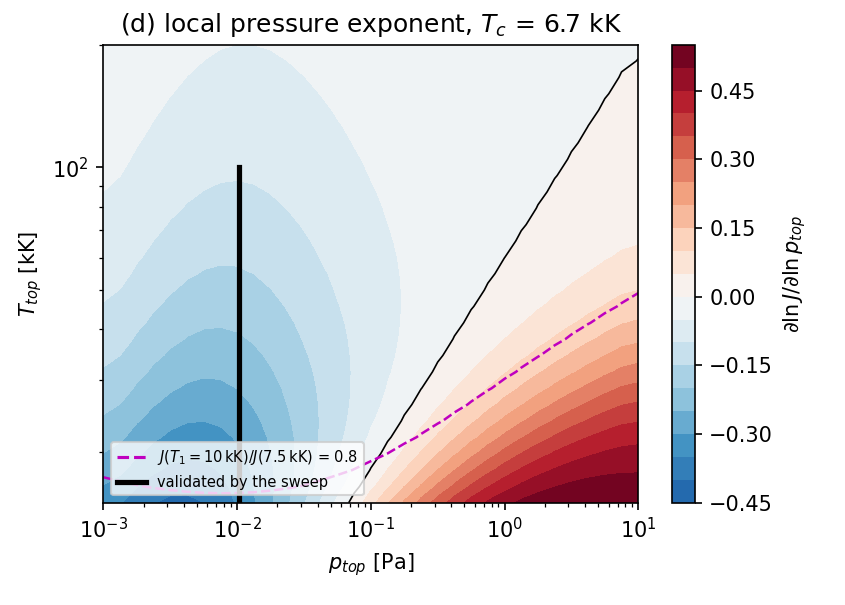
\includegraphics[width=\textwidth]{Jtable_exponent.png}
    \end{column}
    \begin{column}{0.44\textwidth}
      \small
      \begin{itemize}\itemsep8pt
        \item Colour: $\partial\ln J/\partial\ln\ptop$ at $T_c = 6.7$\,kK.
        \item Dashed: $J(T_1{=}10\,\text{kK})/J(7.5\,\text{kK}) = 0.8$.
              Right of it, $J$ depends on the marker.
        \item Black bar: the earlier C7-line validation.
        \item Sweep block: outside, except its edge at 18\,kK
              (marker ratio 0.84 at 0.04\,Pa, 0.79 at 0.08\,Pa).
      \end{itemize}
    \end{column}
  \end{columns}
\end{frame}

\begin{frame}{Backup: sources and reproduction}
  \scriptsize
  \begin{tabular}{@{}ll@{}}
    \toprule
    Claim & Where it comes from \\
    \midrule
    Derivation of $J$, wave phase, contraction &
      \texttt{docs/studies/boundaries/twall\_mass\_flux\_relaxation\_timescales.md} \\
    The analytic table, $T_c$ and marker sensitivity &
      \texttt{docs/studies/boundaries/analytic\_evaporation\_J\_table.md} \\
    The sweep, the classes, the corner follow-up &
      \texttt{docs/studies/boundaries/tp\_sweep\_evaporation\_closure\_validation.md} \\
    $J$ quadrature, Saha EOS, measured $h_c$ and $\LTR$ &
      \texttt{util/twall\_relaxation\_diag.py} (\texttt{j\_theory}, \texttt{analyse}) \\
    Conductivity & \texttt{util/conductive\_flux.py} (matches \texttt{physics.hpp}) \\
    Table & \texttt{util/analytic\_evaporation\_table.py} \\
    \texttt{ISO\_P\_TOP} rebuild & \texttt{scenarios/model\_column.cpp};
      \texttt{docs/doxygen/pages/configuration.md} \\
    Sweep driver and reduction & \texttt{util/run\_tp\_sweep.sh},
      \texttt{util/tp\_sweep\_compare.py}, \\
      & \texttt{util/plot\_tp\_sweep\_vs\_analytic.py} \\
    Corner follow-up & \texttt{util/tp\_corner\_test\_compare.py};
      \texttt{outputs/model\_column/tp\_sweep\_corner/} \\
    Integrand figure & \texttt{util/plot\_J\_integrand.py} \\
    Figure provenance & \texttt{figures/README.md}; \texttt{visualize\_commands.md}
      \S20--22 \\
    \bottomrule
  \end{tabular}
  \vspace{8pt}

  \textbf{Reproduce} (the 6.4\,GB of raw runs stay on the mac-mini):\\[2pt]
  \texttt{SWEEP\_JOBS=4 SWEEP\_THREADS=2 util/run\_tp\_sweep.sh
    outputs/model\_column/tp\_sweep 5000 10}\\
  \texttt{.venv/bin/python util/tp\_sweep\_compare.py --dir
    outputs/model\_column/tp\_sweep --workers 8}\\
  \texttt{.venv/bin/python util/plot\_tp\_sweep\_vs\_analytic.py --dir
    outputs/model\_column/tp\_sweep}\\[4pt]
  Commits: \texttt{247a317} (\texttt{ISO\_P\_TOP}), \texttt{417d31a} (sweep
  comparison).
\end{frame}

\end{document}
